\documentclass{article}
\usepackage[utf8]{inputenc}
\usepackage{amsmath}
\usepackage{amssymb}
\usepackage{wasysym}
\usepackage{amsfonts} 
\usepackage{graphicx}
\usepackage{hyperref}
\usepackage[mathscr]{euscript}
\usepackage{geometry}
\usepackage{subfig}
\usepackage{float}
\geometry{left=2.5cm,right=2.5cm,top=2.5cm,bottom=2.5cm}

\newcommand{\resistor}[1]{$\text{#1} \Omega \text{ Resistor}$}

\title{Soldering Guide \\
\large CHARM}
\author{Martin Michalski}

\begin{document}

\maketitle

% \section{USB-C Port}

% \subsection{Materials}
% Begin by retrieving the components in \autoref{tbl:usbc-materials}.

% \begin{table}[H]
%     \begin{center}
%         \begin{tabular}{ c|c|c|c } 
%             \textbf{Part No.} & \textbf{Description} & \textbf{Silkscreen No(s).} & \textbf{Quantity} \\ 
%             \hline
%             USB4140-GF-0070-C & USB-C Port & J1 & 1 \\ 
%             \hline
%             SF-1206F250-2 & 2.5A Fuse  & F1 & 1 \\ 
%             \hline
%             RT0603DRE075K1L & \resistor{5.1k} & R3,R6 & 2   \\ 
%             \hline
%             RT0603FRE131KL & \resistor{1k} & R5 & 1\\ 
%             \hline
%             150080RS75000 & USB LED & D1 & 1\\ 
%         \end{tabular}
%     \end{center}
%     \caption{Required Components for USB-C Subsystem}
%     \label{tbl:usbc-materials}
% \end{table}

% \subsection{Layout}

% Reference \autoref{fig:usbc-layout} to properly place the components.

% \begin{figure}[H]
%     \centering
%         \subfloat[\centering Soldered Example]{{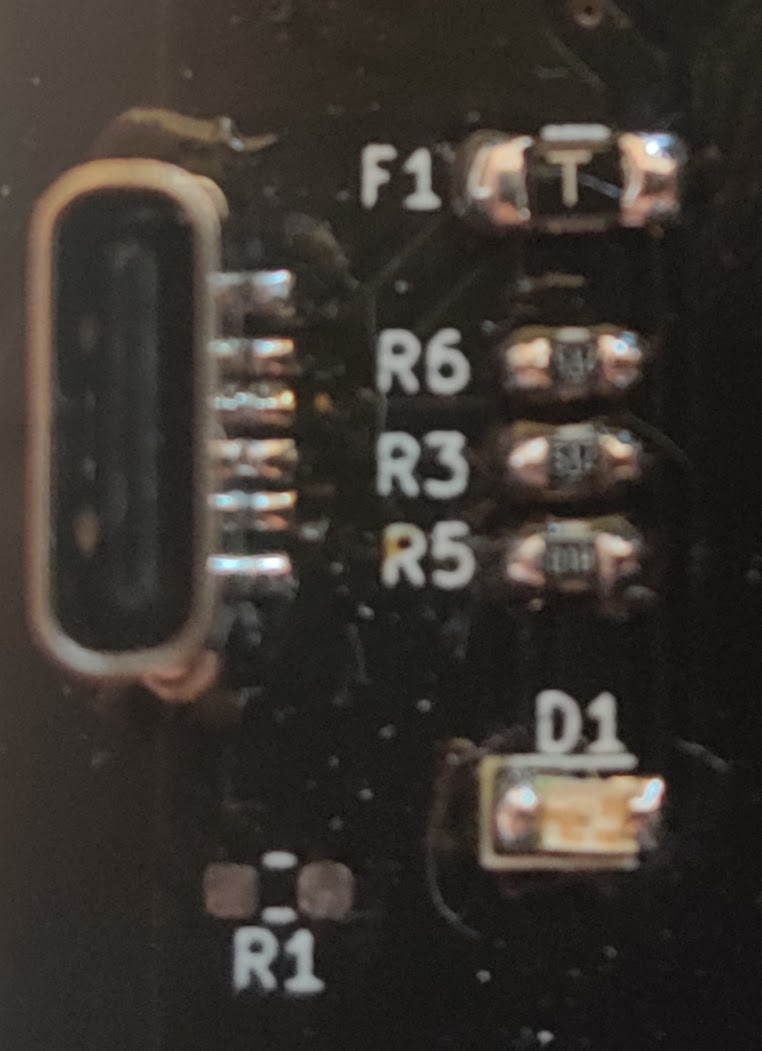
\includegraphics[height=6cm]{./images/usb_real.jpg} }}%
%         \qquad
%         \subfloat[\centering PCB Layout]{{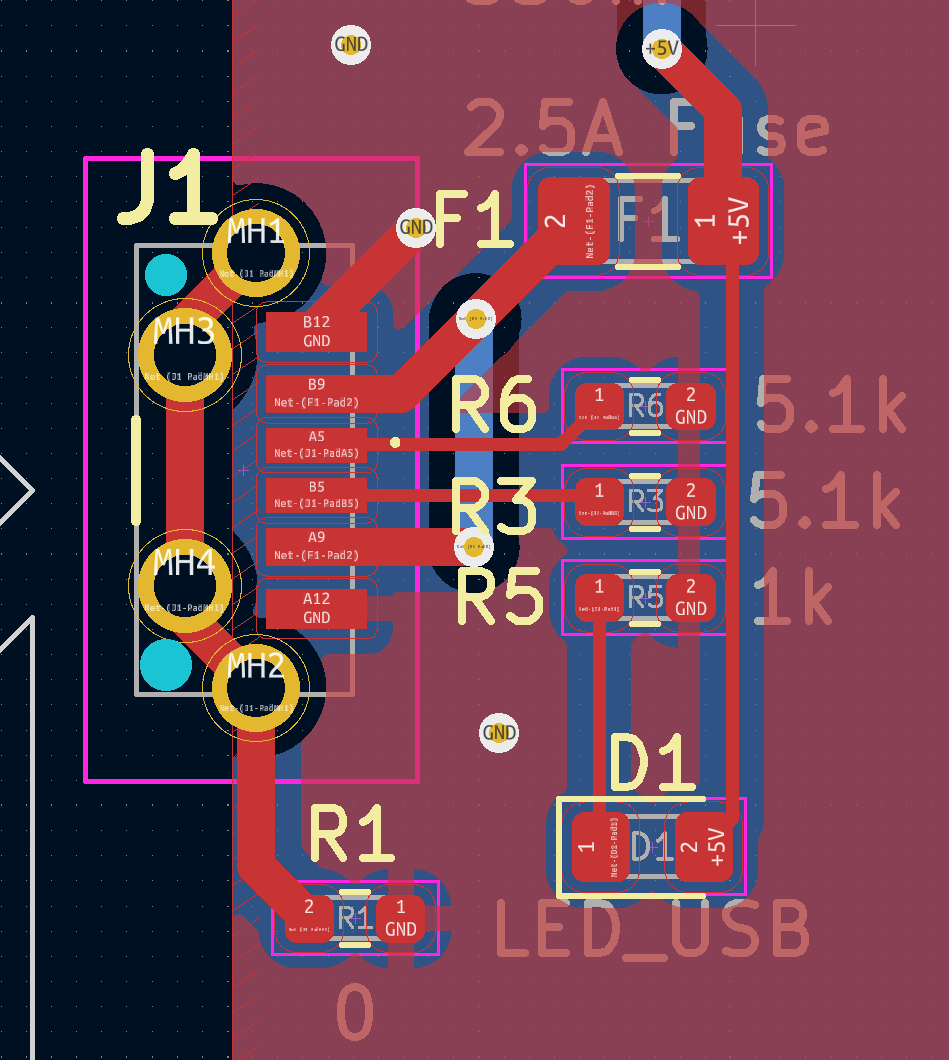
\includegraphics[height=6cm]{./images/usb_pcb_kicad.png} }}%
%         \caption{USB-C Subsystem Layout Reference}%
%     \label{fig:usbc-layout}%
% \end{figure}

% \noindent \textbf{Polarity Notes}\\
% \noindent \textit{Pay special attention to the orientation of the following components}
% \begin{itemize}
%   \item D1: USB LED (Arrow should point towards the USB-C Port)
% \end{itemize}

% \subsection{Soldering}

% Solder the components. \\

% \noindent \textbf{Recommended Order}

% \begin{enumerate}
%   \item F1: 2.5A Fuse
%   \item R6: \resistor{5.1k}
%   \item R3: \resistor{5.1k}
%   \item R5: \resistor{1k}
%   \item D1: USB LED
%   \item J1: USB-C Port
% \end{enumerate}

% \noindent \textit{Do not solder R1.}

% \subsection{Quality Assurance}

% \section{Boost Converter}

% \subsection{Materials}
% Begin by retrieving the components in \autoref{tbl:boost-materials}.

% \begin{figure}[H]
%     \begin{center}
%         \begin{tabular}{ c|c|c|c } 
%             \textbf{Part No.} & \textbf{Description} & \textbf{Silkscreen No(s).} & \textbf{Quantity} \\ 
%             \hline
%             LM2585S-12/NOPB & Boost Converter IC & IC3 & 1 \\ 
%             \hline
%             UUD1C221MCL1GS & 220uF Capacitor & C7 & 1 \\ 
%             \hline
%             16SVPF1000M & 1mF Capacitor & C9 & 1 \\ 
%             \hline
%             ECPU1C334MA5 & 330nF Capacitor & C2 & 1 \\ 
%             \hline
%             MSS1210-683MED & 68uH Inductor & L2 & 1 \\ 
%             \hline
%             RC0603FR-072K94L & \resistor{2.94k} & R7 & 1 \\
%             \hline
%             SS24FL & Schottky Diode & D4 & 1 
%         \end{tabular}
%     \end{center}
%     \caption{Required Components for Boost Converter Subsystem}
%     \label{tbl:boost-materials}
% \end{figure}

% \subsection{Layout}

% Reference \autoref{fig:boost-layout} to properly place the components.

% \begin{figure}[H]
%     \centering
%         \subfloat[\centering Soldered Example]{{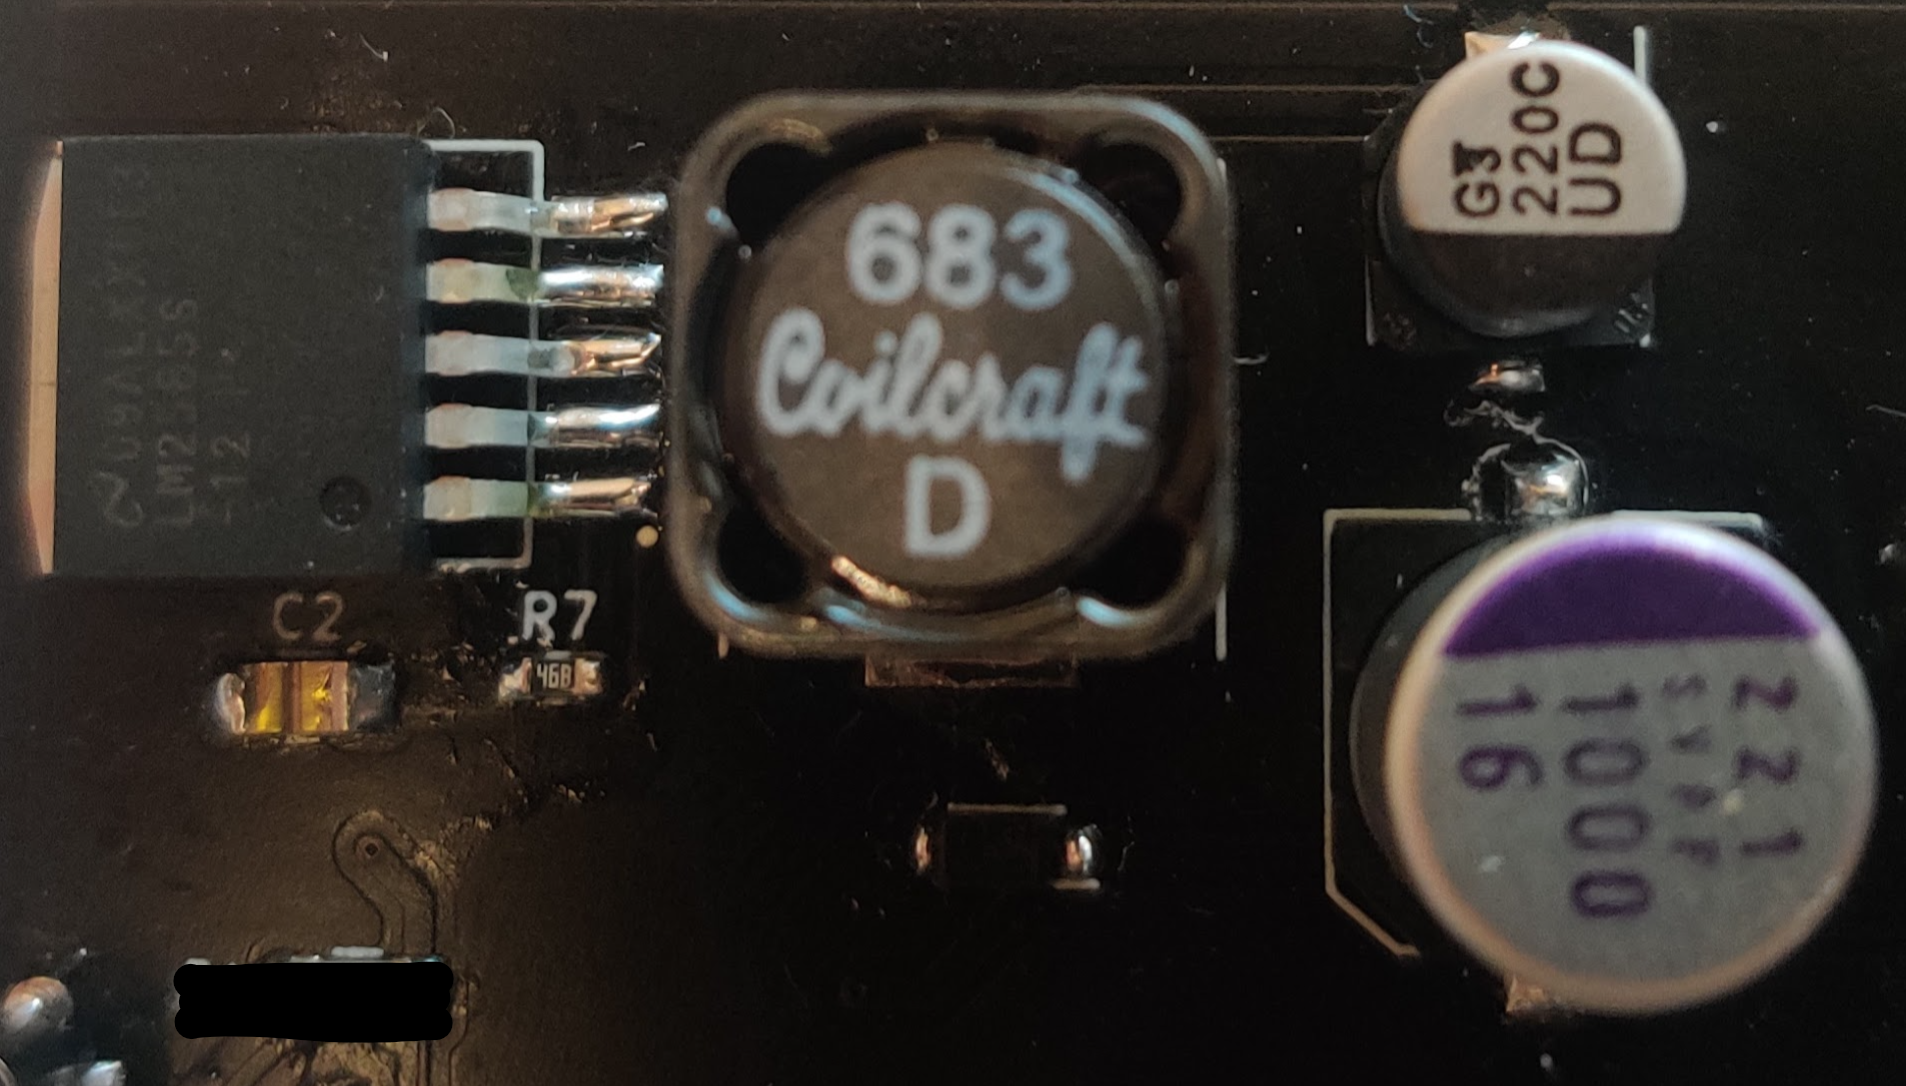
\includegraphics[height=4.5cm]{./images/boost_real.png} }}%
%         \qquad
%         \subfloat[\centering PCB Layout]{{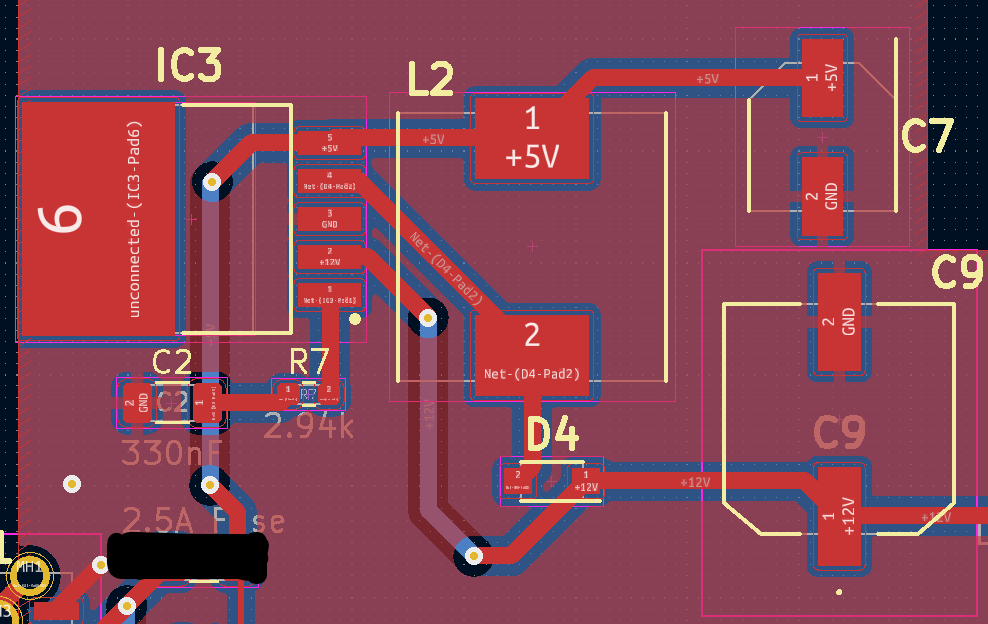
\includegraphics[height=4.5cm]{./images/boost_pcb_kicad.png} }}%
%         \caption{Boost Converter Subsystem Layout Reference}%
%     \label{fig:boost-layout}%
% \end{figure}

% \noindent \textbf{Polarity Notes}\\
% \noindent \textit{Pay special attention to the orientation of the following components}
% \begin{itemize}
%   \item C9: 1mF Capacitor (Reference \autoref{fig:boost-layout}.a)
%   \item C7: 220uF Capacitor (Reference \autoref{fig:boost-layout}.a)
%   \item C2: TODO TREVOR
%   \item D4: TODO TREVOR
% \end{itemize}

% \subsection{Soldering}

% Solder the components. \\

% \noindent \textbf{Recommended Order}

% \begin{enumerate}
%   \item IC3: Boost Converter IC 
%   \item C2: 330nF Capacitor
%   \item R7: \resistor{2.94k}
%   \item D4: Schottky Diode 
%   \item L2: 68uH Inductor
%   \item C7: 1mF Capacitor
%   \item C9: 220uF Capacitor
% \end{enumerate}

% \subsection{Quality Assurance}

% \section{Battery Charge Controller}

% \subsection{Materials}
% Begin by retrieving the components in \autoref{tbl:charge-materials}.

% \begin{figure}[H]
%     \begin{center}
%         \begin{tabular}{ c|c|c|c } 
%             \textbf{Part No.} & \textbf{Description} & \textbf{Silkscreen No(s).} & \textbf{Quantity} \\ 
%             \hline
%             MCP73844-840I/MS & Battery Charge IC & IC1 & 1 \\ 
%             \hline
%             EEE-FN1E100R & 10uF Capacitor & C1, C6 & 2 \\ 
%             \hline
%             T491A104K035AT & 0.1uF Capacitor & C3 & 1 \\ 
%             \hline
%             RT0603BRD0750KL & \resistor{50k} & R2 & 1 \\ 
%             \hline
%             ERJ-6RQFR22V & \resistor{220m} & R4 & 1 \\ 
%             \hline
%             150080RS75000 & Red LED & D2 &  1 \\ 
%             \hline
%             IRF7404TRPBF & MOSFET & Q1 & 1 \\ 
%             \hline
%             MCP73844-840I/MS & Battery Holder & J2 & 1 \\ 
%             \hline
%             L101011MS02Q & Switch & SW1 & 1 
%         \end{tabular}
%     \end{center}
%     \caption{Required Components for the Battery Charge Controller Subsystem}
%     \label{tbl:charge-materials}
% \end{figure}

% \subsection{Layout}

% Reference \autoref{fig:charge-layout} to properly place the components.

% \begin{figure}[H]
%     \centering
%         \subfloat[\centering Soldered Example]{{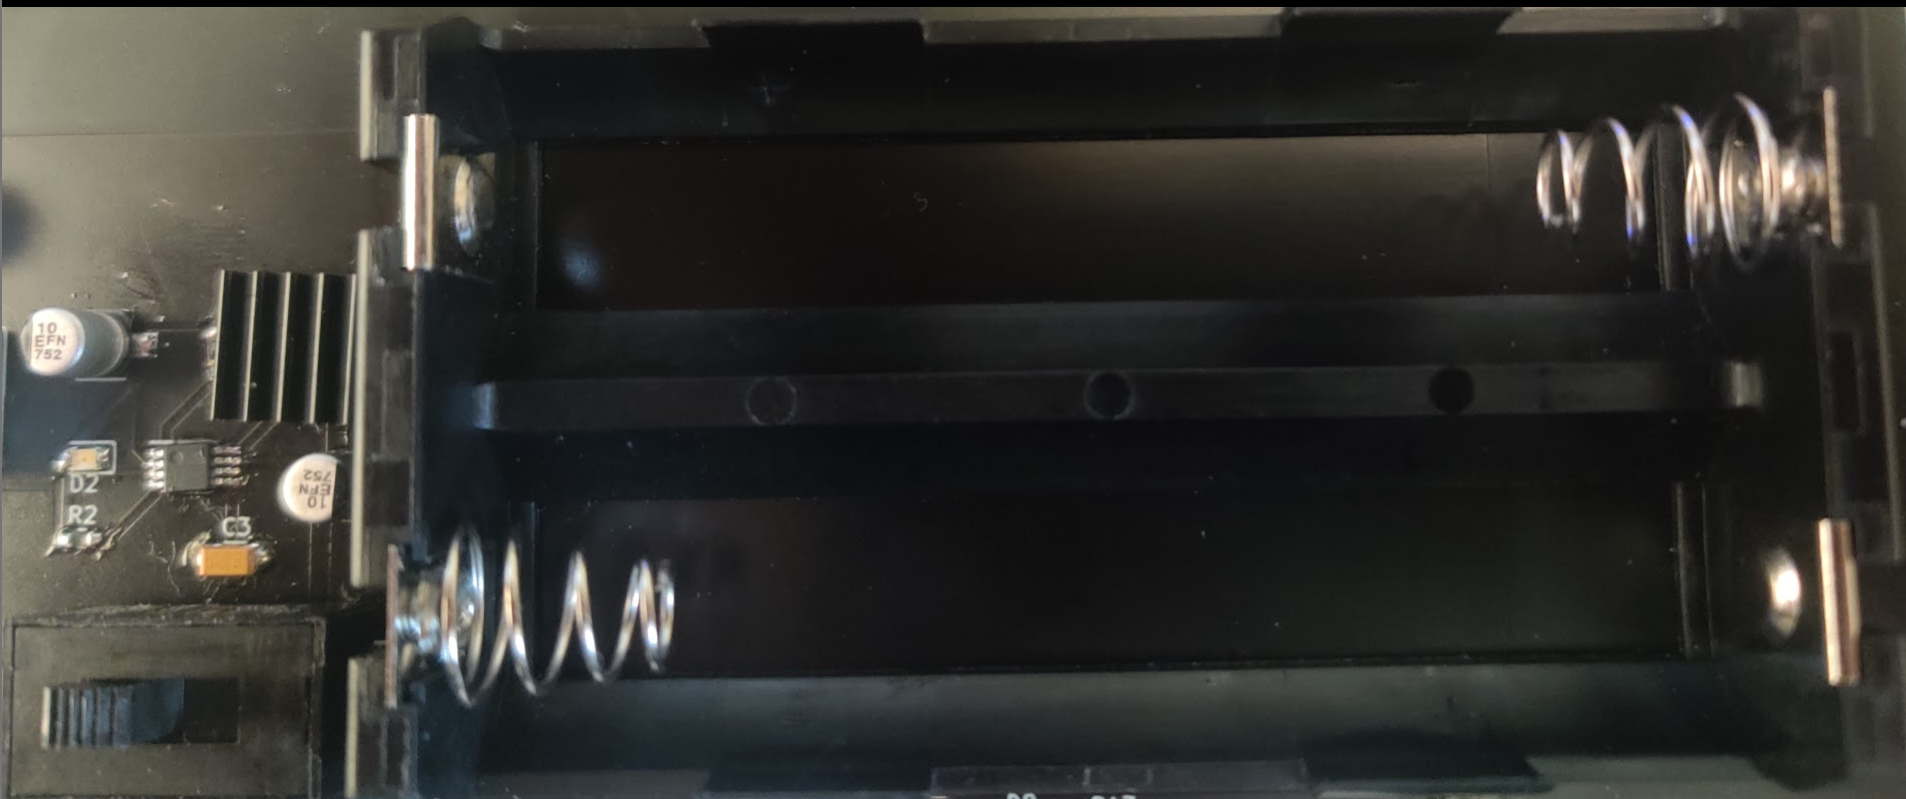
\includegraphics[height=6cm]{./images/charge_real.png} }}%
%         \qquad
%         \subfloat[\centering PCB Layout]{{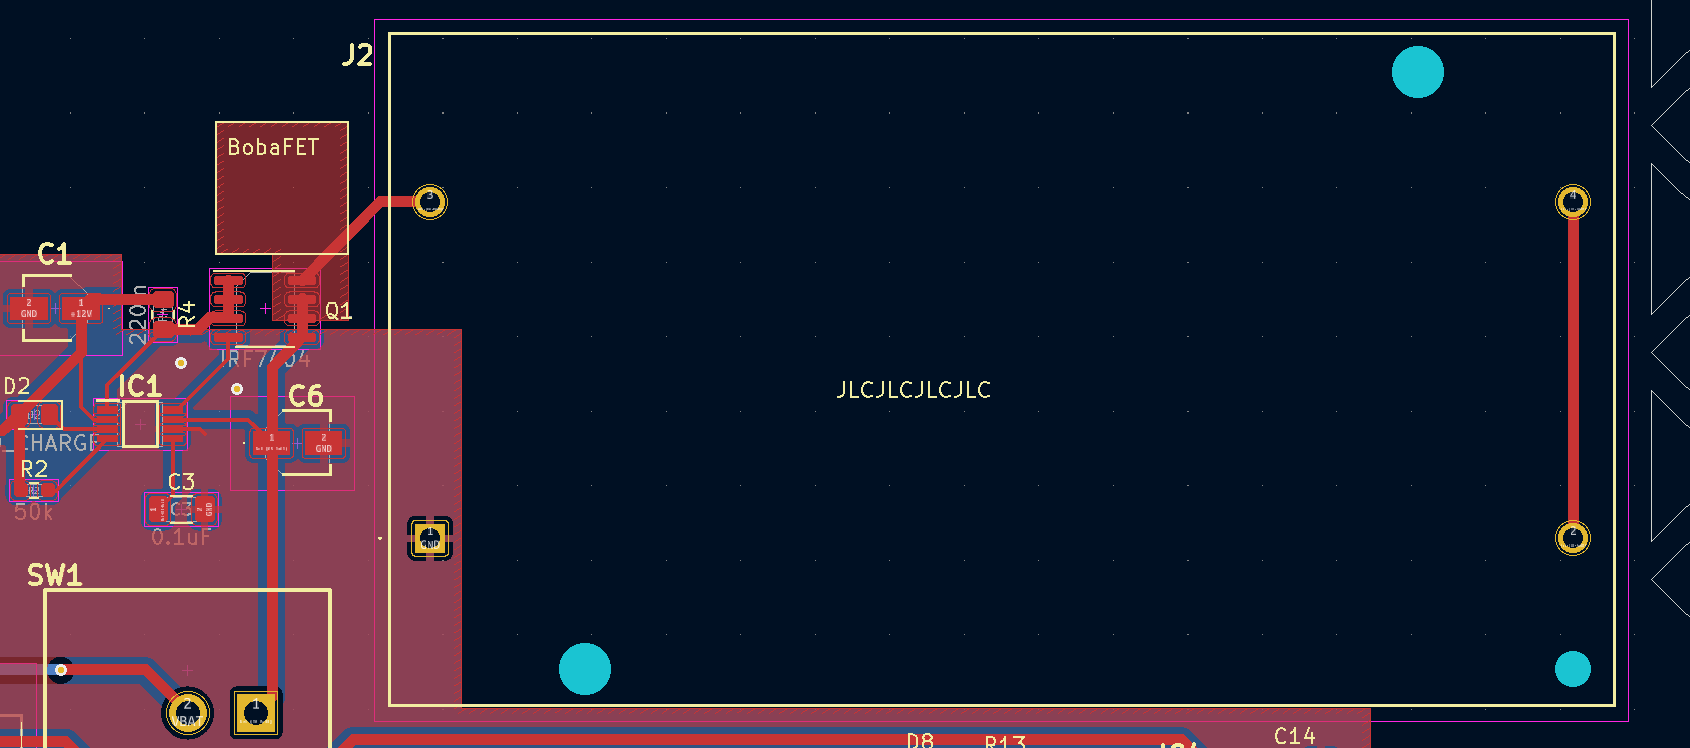
\includegraphics[height=6cm]{./images/charge_pcb_kicad.png} }}%
%         \caption{Battery Charge Controller Subsystem Layout Reference}%
%     \label{fig:charge-layout}%
% \end{figure}

% \noindent \textbf{Polarity Notes}\\
% \noindent \textit{Pay special attention to the orientation of the following components}
% \begin{itemize}
%   \item C1: 10uF Capacitor (Reference \autoref{fig:charge-layout}.a)
%   \item C6: 10uF Capacitor (Reference \autoref{fig:charge-layout}.a)
%   \item C3: 0.1uF Capacitor  (Banded, bevelled side away from J2, Battery Holder)
%   \item D2: Red LED (Arrow towards IC1)
%   \item IC1: Battery Charge IC (Dot in top-left corner, towards H1 board corner)
%   \item Q1: TODO TREVOR
% \end{itemize}

% \subsection{Soldering}

% Solder the components. \\

% \noindent \textbf{Recommended Order}

% \begin{enumerate}
%   \item IC1: Battery Charge IC
%   \item Q1: MOSFET
%   \item R4: \resistor{220m} 
%   \item D2: Red LED
%   \item R2: \resistor{50k}
%   \item C3: 0.1uF Capacitor
%   \item C1, C6: 10uF Capacitors 
%   \item SW1: Switch
%   \item J2: Battery Holder
% \end{enumerate}

% \subsection{Quality Assurance}

\section{Buck Converter}

\subsection{Materials}
Begin by retrieving the components in TODO.

\begin{figure}[H]
    \begin{center}
        \begin{tabular}{ c|c|c|c } 
            \textbf{Part No.} & \textbf{Description} & \textbf{Silkscreen No(s).} & \textbf{Quantity} \\ 
            \hline
            USB4140-GF-0070-C & USB-C Port & J1 & 1 \\ 
        \end{tabular}
    \end{center}
    \caption{Required Components for USB-C Subsystem}
    \label{tbl:TODO-materials}
\end{figure}

\subsection{Layout}

\begin{figure}[H]
    \centering
        \subfloat[\centering Soldered Example]{{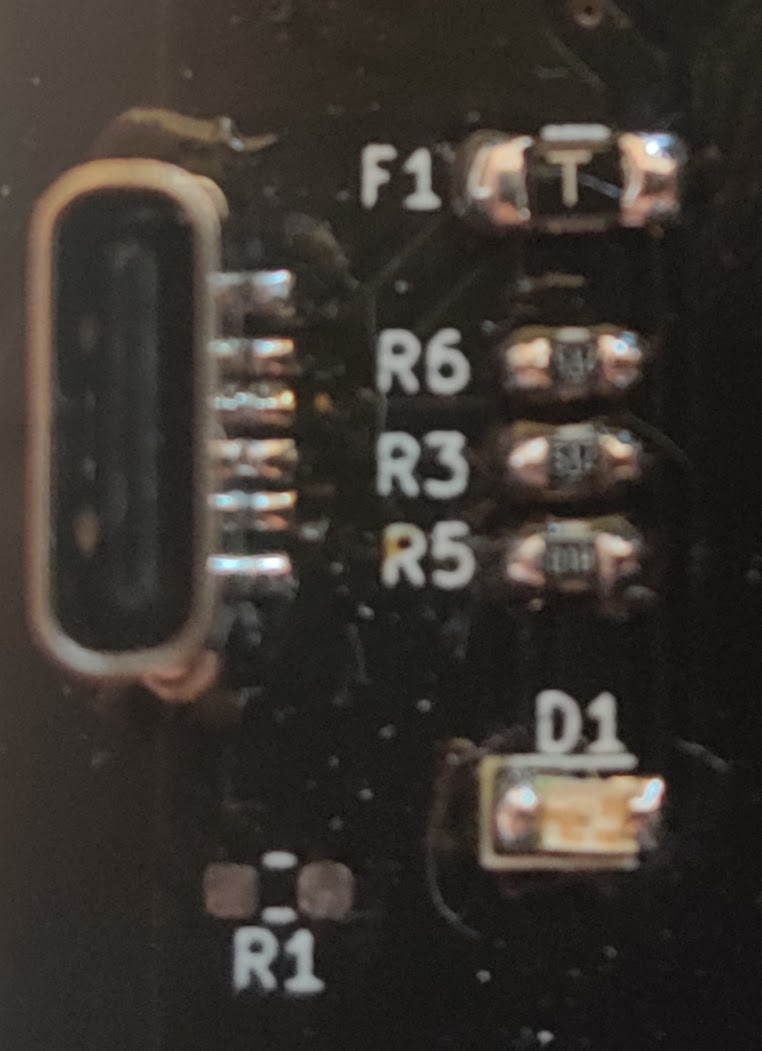
\includegraphics[height=6cm]{./images/usb_real.jpg} }}%
        \qquad
        \subfloat[\centering PCB Layout]{{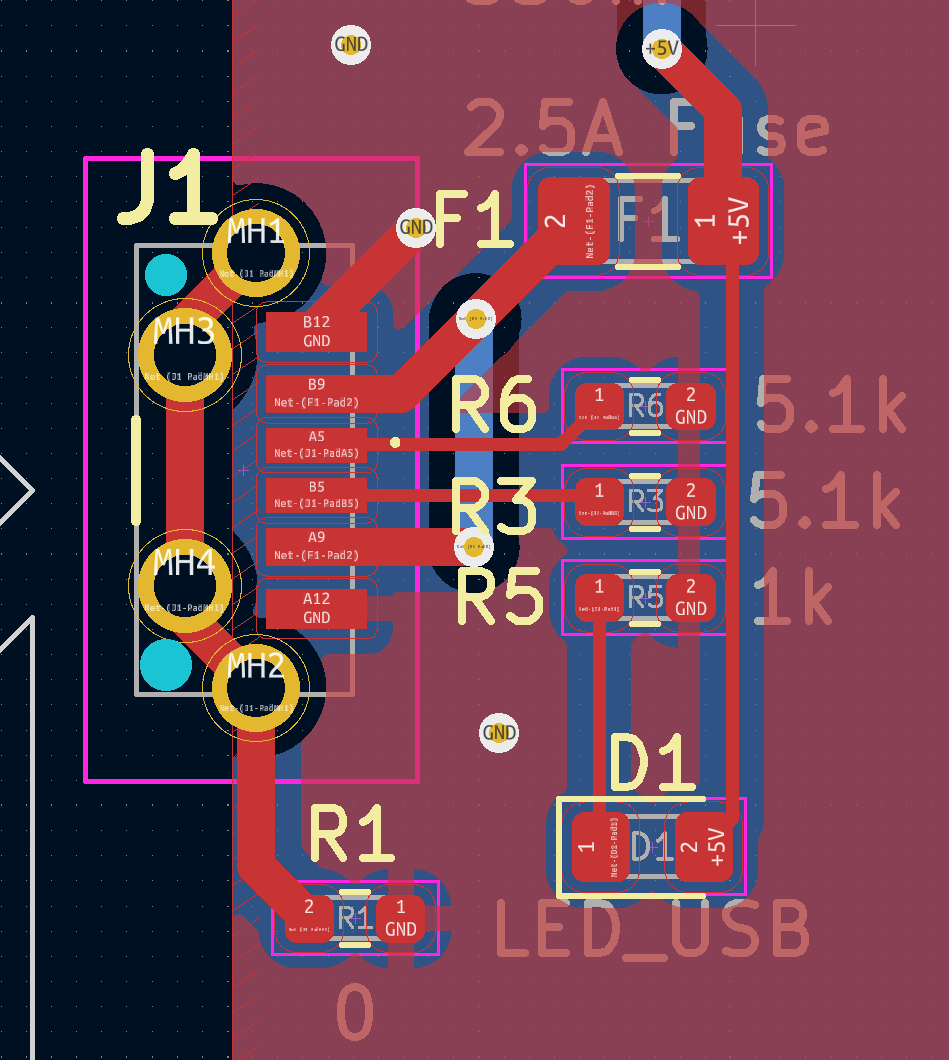
\includegraphics[height=6cm]{./images/usb_pcb_kicad.png} }}%
        \caption{TODO Subsystem Layout Reference}%
    \label{fig:TODO-layout}%
\end{figure}

\noindent \textbf{Polarity Notes}\\
\noindent \textit{Pay special attention to the orientation of the following components}
\begin{itemize}
  \item D1: USB LED
\end{itemize}

\subsection{Soldering}

Solder the components. \\

\noindent \textbf{Recommended Order}

\begin{enumerate}
  \item X1: X1 Description
\end{enumerate}
\subsection{Quality Assurance}

\section{Omega 2S+}

\subsection{Materials}
Begin by retrieving the components in TODO.

\begin{figure}[H]
    \begin{center}
        \begin{tabular}{ c|c|c|c } 
            \textbf{Part No.} & \textbf{Description} & \textbf{Silkscreen No(s).} & \textbf{Quantity} \\ 
            \hline
            USB4140-GF-0070-C & USB-C Port & J1 & 1 \\ 
        \end{tabular}
    \end{center}
    \caption{Required Components for USB-C Subsystem}
    \label{tbl:TODO-materials}
\end{figure}

\subsection{Layout}

\begin{figure}[H]
    \centering
        \subfloat[\centering Soldered Example]{{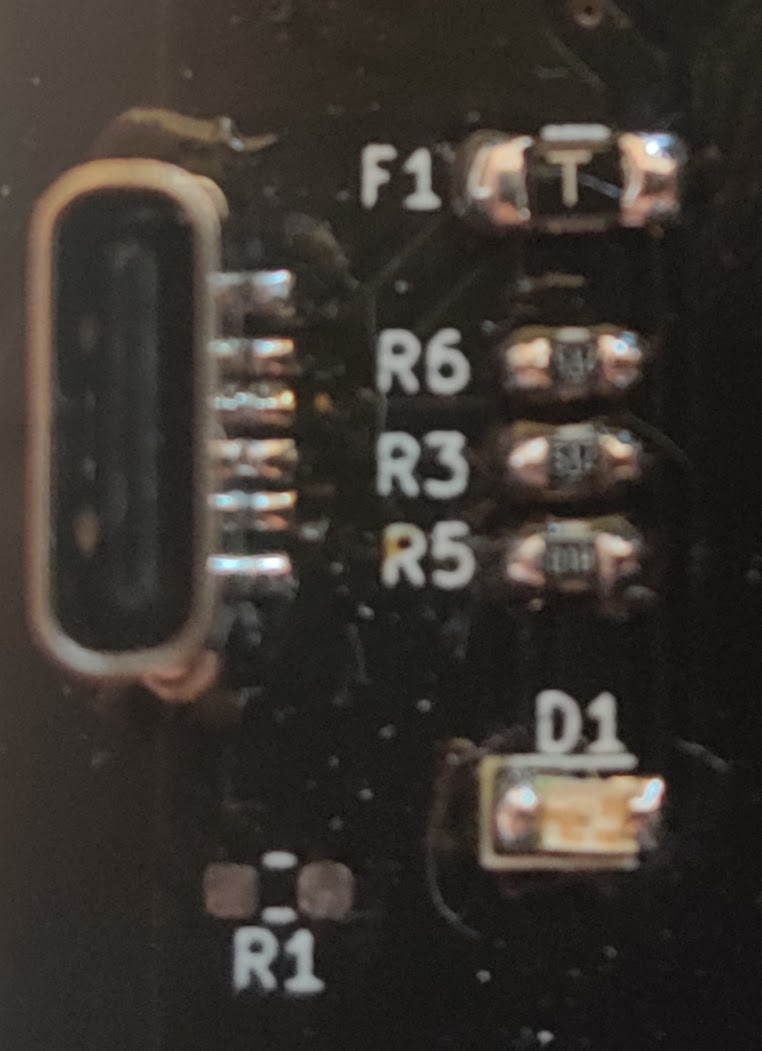
\includegraphics[height=6cm]{./images/usb_real.jpg} }}%
        \qquad
        \subfloat[\centering PCB Layout]{{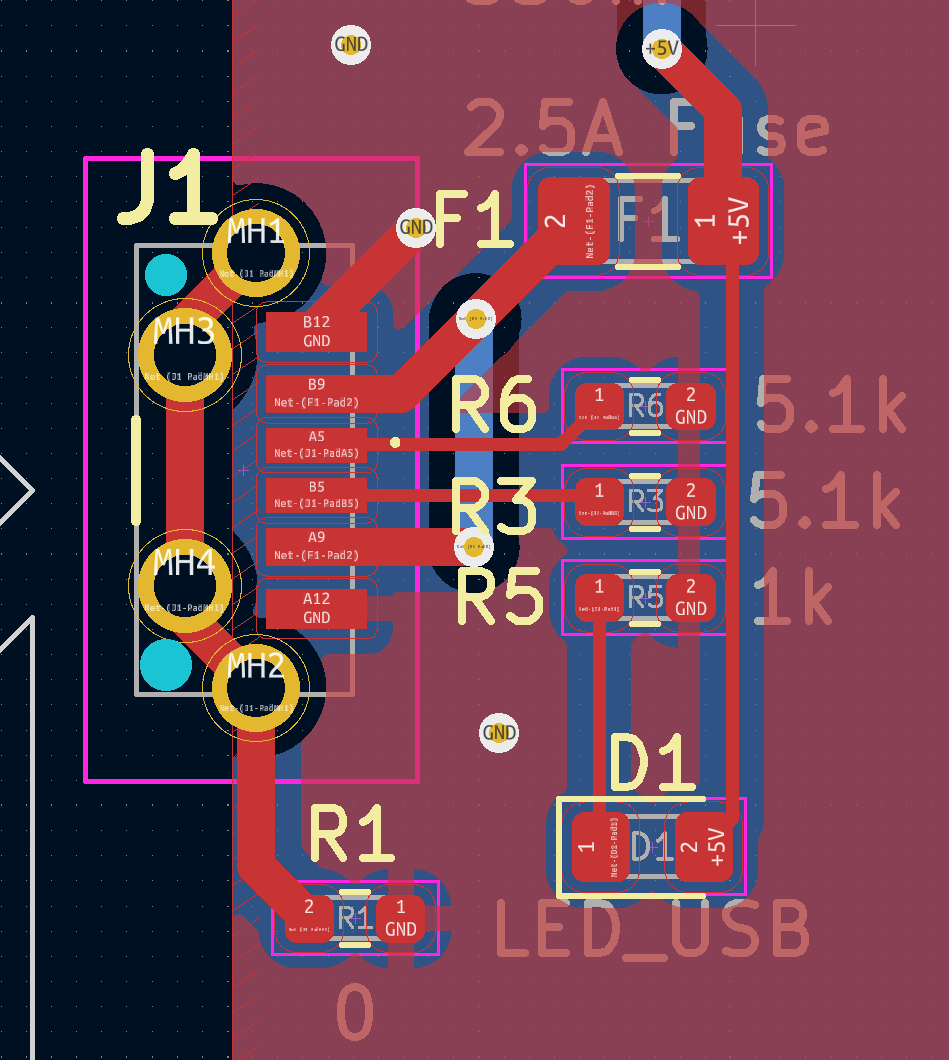
\includegraphics[height=6cm]{./images/usb_pcb_kicad.png} }}%
        \caption{TODO Subsystem Layout Reference}%
    \label{fig:TODO-layout}%
\end{figure}

\noindent \textbf{Polarity Notes}\\
\noindent \textit{Pay special attention to the orientation of the following components}
\begin{itemize}
  \item D1: USB LED
\end{itemize}

\subsection{Soldering}

Solder the components. \\

\noindent \textbf{Recommended Order}

\begin{enumerate}
  \item X1: X1 Description
\end{enumerate}
\subsection{Quality Assurance}

\section{GPS Module}

\subsection{Materials}
Begin by retrieving the components in TODO.

\begin{figure}[H]
    \begin{center}
        \begin{tabular}{ c|c|c|c } 
            \textbf{Part No.} & \textbf{Description} & \textbf{Silkscreen No(s).} & \textbf{Quantity} \\ 
            \hline
            USB4140-GF-0070-C & USB-C Port & J1 & 1 \\ 
        \end{tabular}
    \end{center}
    \caption{Required Components for USB-C Subsystem}
    \label{tbl:TODO-materials}
\end{figure}

\subsection{Layout}

\begin{figure}[H]
    \centering
        \subfloat[\centering Soldered Example]{{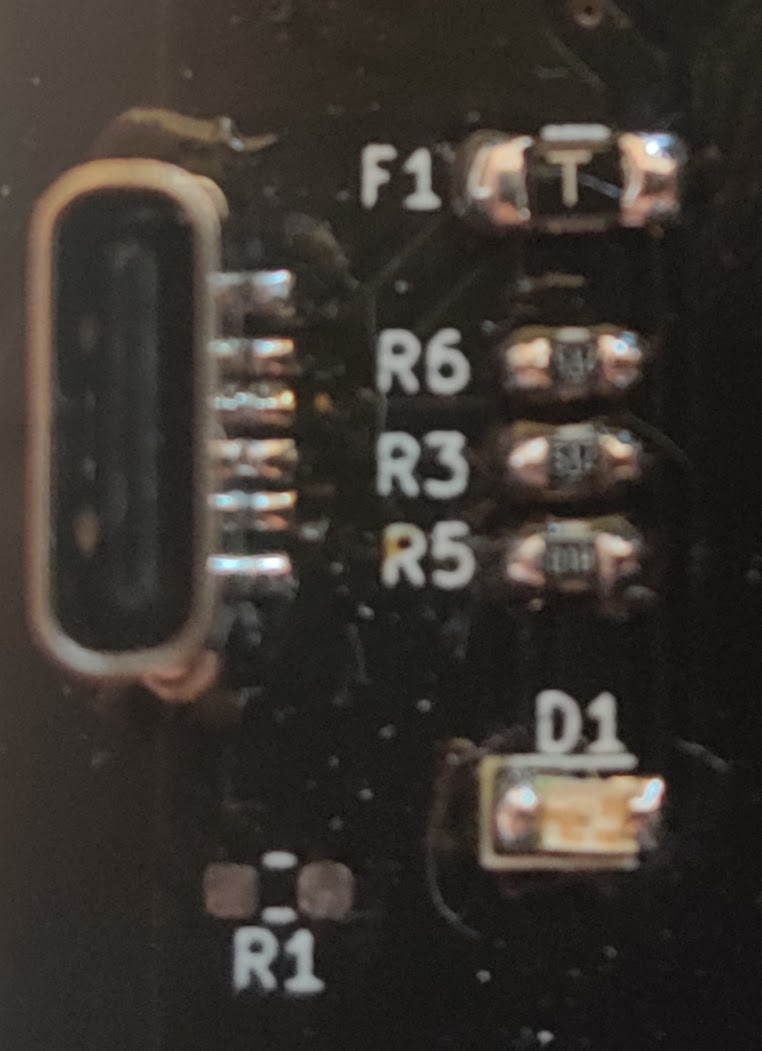
\includegraphics[height=6cm]{./images/usb_real.jpg} }}%
        \qquad
        \subfloat[\centering PCB Layout]{{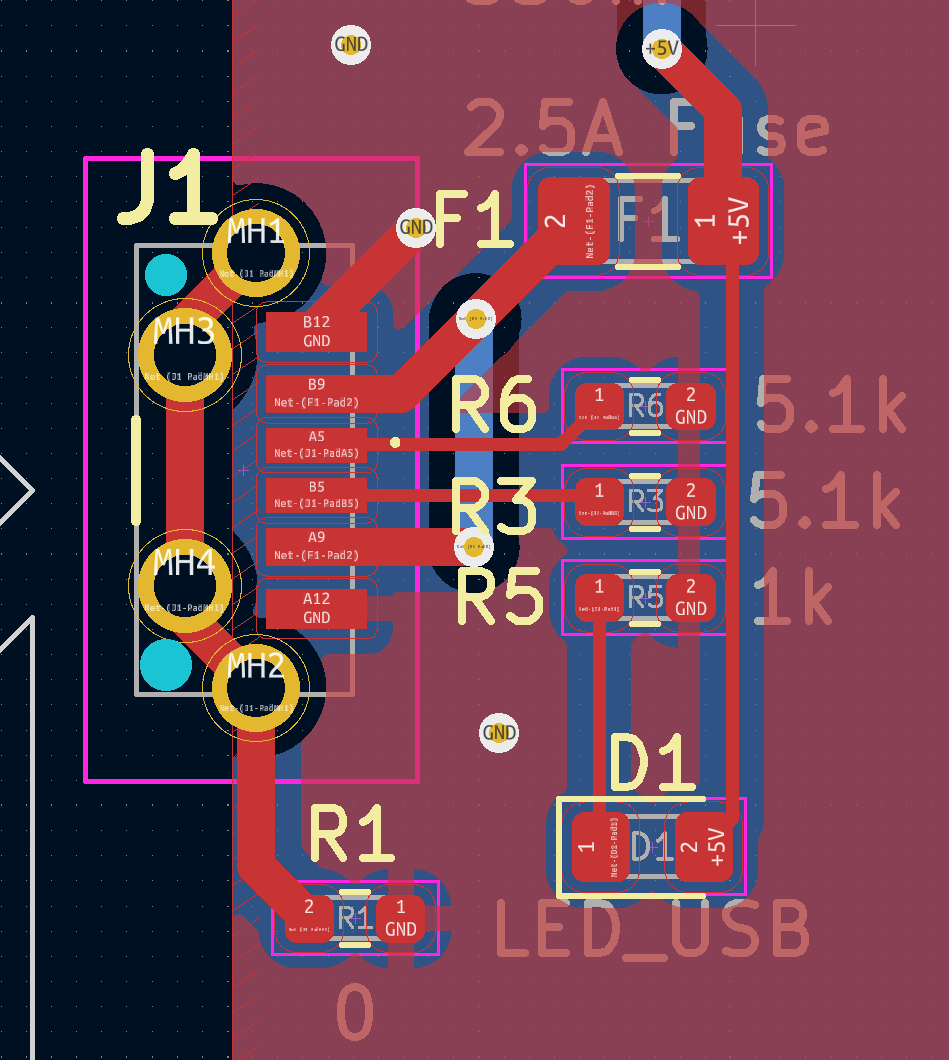
\includegraphics[height=6cm]{./images/usb_pcb_kicad.png} }}%
        \caption{TODO Subsystem Layout Reference}%
    \label{fig:TODO-layout}%
\end{figure}

\noindent \textbf{Polarity Notes}\\
\noindent \textit{Pay special attention to the orientation of the following components}
\begin{itemize}
  \item D1: USB LED
\end{itemize}

\subsection{Soldering}

Solder the components. \\

\noindent \textbf{Recommended Order}

\begin{enumerate}
  \item X1: X1 Description
\end{enumerate}
\subsection{Quality Assurance}

\section{Battery Monitor}

\subsection{Materials}
Begin by retrieving the components in TODO.

\begin{figure}[H]
    \begin{center}
        \begin{tabular}{ c|c|c|c } 
            \textbf{Part No.} & \textbf{Description} & \textbf{Silkscreen No(s).} & \textbf{Quantity} \\ 
            \hline
            USB4140-GF-0070-C & USB-C Port & J1 & 1 \\ 
        \end{tabular}
    \end{center}
    \caption{Required Components for USB-C Subsystem}
    \label{tbl:TODO-materials}
\end{figure}

\subsection{Layout}

\begin{figure}[H]
    \centering
        \subfloat[\centering Soldered Example]{{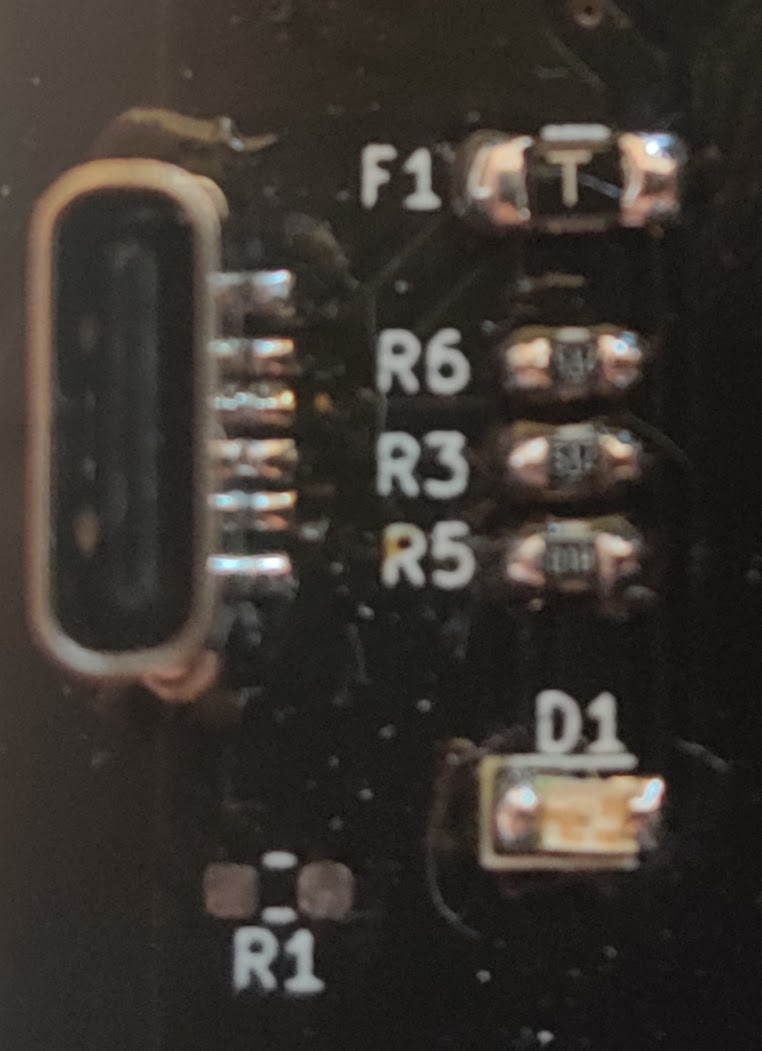
\includegraphics[height=6cm]{./images/usb_real.jpg} }}%
        \qquad
        \subfloat[\centering PCB Layout]{{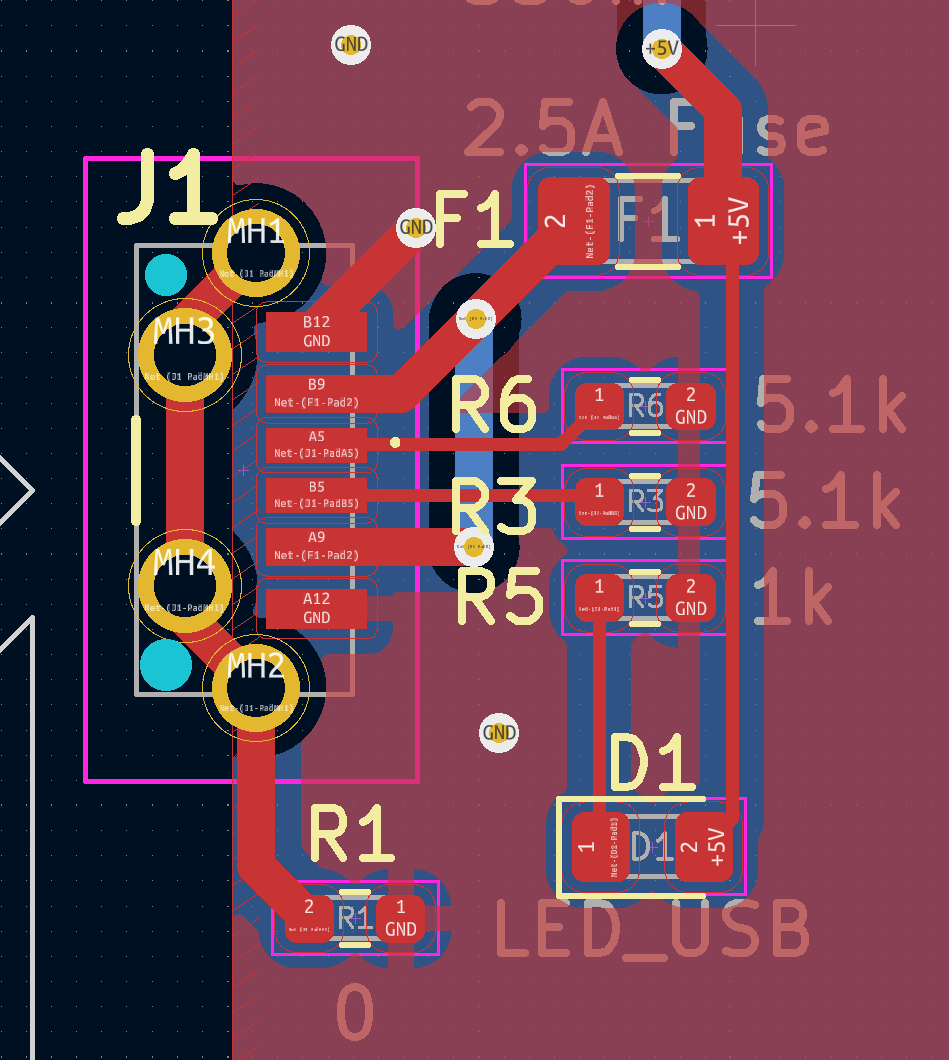
\includegraphics[height=6cm]{./images/usb_pcb_kicad.png} }}%
        \caption{TODO Subsystem Layout Reference}%
    \label{fig:TODO-layout}%
\end{figure}

\noindent \textbf{Polarity Notes}\\
\noindent \textit{Pay special attention to the orientation of the following components}
\begin{itemize}
  \item D1: USB LED
\end{itemize}

\subsection{Soldering}

Solder the components. \\

\noindent \textbf{Recommended Order}

\begin{enumerate}
  \item X1: X1 Description
\end{enumerate}
\subsection{Quality Assurance}

\end{document}